\documentclass{article}
\usepackage{amsmath}
\usepackage[utf8]{inputenc}
\usepackage{natbib}
\bibliographystyle{abbrvnat}
\setcitestyle{authoryear,open={((},close={))}}
\usepackage{graphicx}
\usepackage{float}
\usepackage[margin=1in]{geometry}

\title{MTH 5315 NUMERICAL METHODS FOR PDE \\ HOMEWORK 3}

\date{\today}
\author{\Huge Max Le \\ \\ ID: 901223283}
\begin{document}
\maketitle
\newpage
\tableofcontents
\newpage
\listoffigures
\newpage

\section{Introduction}
\subsection{Problem statement}
For this assignment, we are given the following 1D Poisson equation to solve: 
\\

\begin{equation}
u_{xx} = 1-2x^2
\end{equation}
\noindent
on the interval from 0 to 1. The boundary conditions are: $u'(0) = 1$ and $u(1) = 0$ at the ends. We are asked to solve the problem using three methods: Gauss Seidel,Conjugate Gradient Method without Preconditioner, and Conjugate Gradient Method with Incomplete Cholesky Decomposition until a residual error of $10^{-4}$ is obtained. The results are plotted and the convergent analysis is performed for each case. An analytical solution is also obtained via the following procedure: \\

\begin{align*}
u_{xx}(x) &= 1-2x^2 \\
\dfrac{d}{dx}(u_x(x))&= 1-2x^2\\
u_x(x)&= \int_{0}^{x} (1-2x^2) dx\\
&=x-\dfrac{2x^3}{3}+C1\\
u(x) &= \int_{0}^{x} (x-\dfrac{2x^3}{3}+C1) dx\\
&=\dfrac{x^2}{2} - \dfrac{x^4}{6} + C1x + C2\\
\textrm{Applying the boundary conditions}\\
u(x) &=  \dfrac{x^2}{2} - \dfrac{x^4}{6} - \dfrac{1}{3}
\end{align*}
\subsection{Stencil}
In order to solve this PDE numerically, we must discretize it using a 2nd order central difference: 

\begin{equation*}
u_{xx} \approx \dfrac{u_{j+1}-2U_j+U_{j-1}}{\Delta x^2}
\end{equation*}

\noindent
This finite difference equation, when combine together with our original PDE, can be written in the form of a linear algebra system. 

\[
\dfrac{1}{\Delta x^2}\begin{bmatrix}
2 & 1 & 0 & \dots & 0 \\
1 & -2 & 1 & \dots & 0 \\
0 & 1 & -2 & 1 & \dots \\
\dots  & \dots  & \dots  & \dots & \dots  \\
\dots & \dots & \dots & \dots & \dots 
\end{bmatrix}
\begin{bmatrix}
u_1 \\ u_2 \\ u_3 \\ \dots \\ u_n 
\end{bmatrix}
=
\begin{bmatrix}
f_1 \\ f_2 \\ f_3 \\ \dots \\ f_n 
\end{bmatrix}
\]

\noindent
This system can be written as: Au = f. Because our boundary condition requires Dirichlet at the end and Neumann at the front, we need to extend our grid by making ghost nodes.  For the Dirichlet boundary condition (U(1) = 0), we begin by substituting into the discretized formula, assume j = N

\begin{align*}
\dfrac{u_{N+1}-2U_N+U_{N-1}}{\Delta x^2} &= f_{N+1}\\
\dfrac{U_{N+1-2U_N}}{\Delta x^2} &= f_{N+1} - \dfrac{U_{N-1}}{\Delta x^2}
\end{align*}


This tells us that to include the ghost node, at the end, the last diagonal element is -2. Likewise, for the Neumann boundary condition, we apply a center difference for the node U1 and U0 (ghost node), this gets the first point of the diagonal to be 2.  Below is the revised system, with ghost points. 

\[
\dfrac{1}{\Delta x^2}\begin{bmatrix}
2&-2& 1 & 0 & \dots & 0 \\
0&1 & -2 & 1 & \dots & 0 \\
0&0 & 1 & -2 & 1 & \dots \\
\dots  & \dots  & \dots  & \dots & \dots & \dots  \\
\dots & \dots & \dots & \dots & \dots & 2
\end{bmatrix}
\begin{bmatrix}
u_0 \\ u_1 \\ u_2 \\ \dots \\ u_n 
\end{bmatrix}
=
\begin{bmatrix}
f_0 \\ f_1 \\ f_2 \\ \dots \\ f_n 
\end{bmatrix}
\]

\newpage
\section{Gauss Seidel}

For this method, we assume that the matrix A can be decomposed into: A = L + U+D, where L = lower triangular matrix and U = upper triangular matrix and D = matrix whose diagonal belongs to A. Then, we can write: 

\begin{align*}
\vec{u}^{\,k+1} &= \vec{u}^{\,k} + \vec{B}^{\,-1}\vec{r}^{\,k}\\
\vec{u}^{\,k+1} &= \vec{u}^{\,k} + (\vec{D}+\vec{L})^-1(\vec{f}-\vec{A}\vec{u}^k)
\end{align*}

\noindent
where B = L + D

\subsection{Results}

Below are results for this method: 


	\begin{figure}[H]
	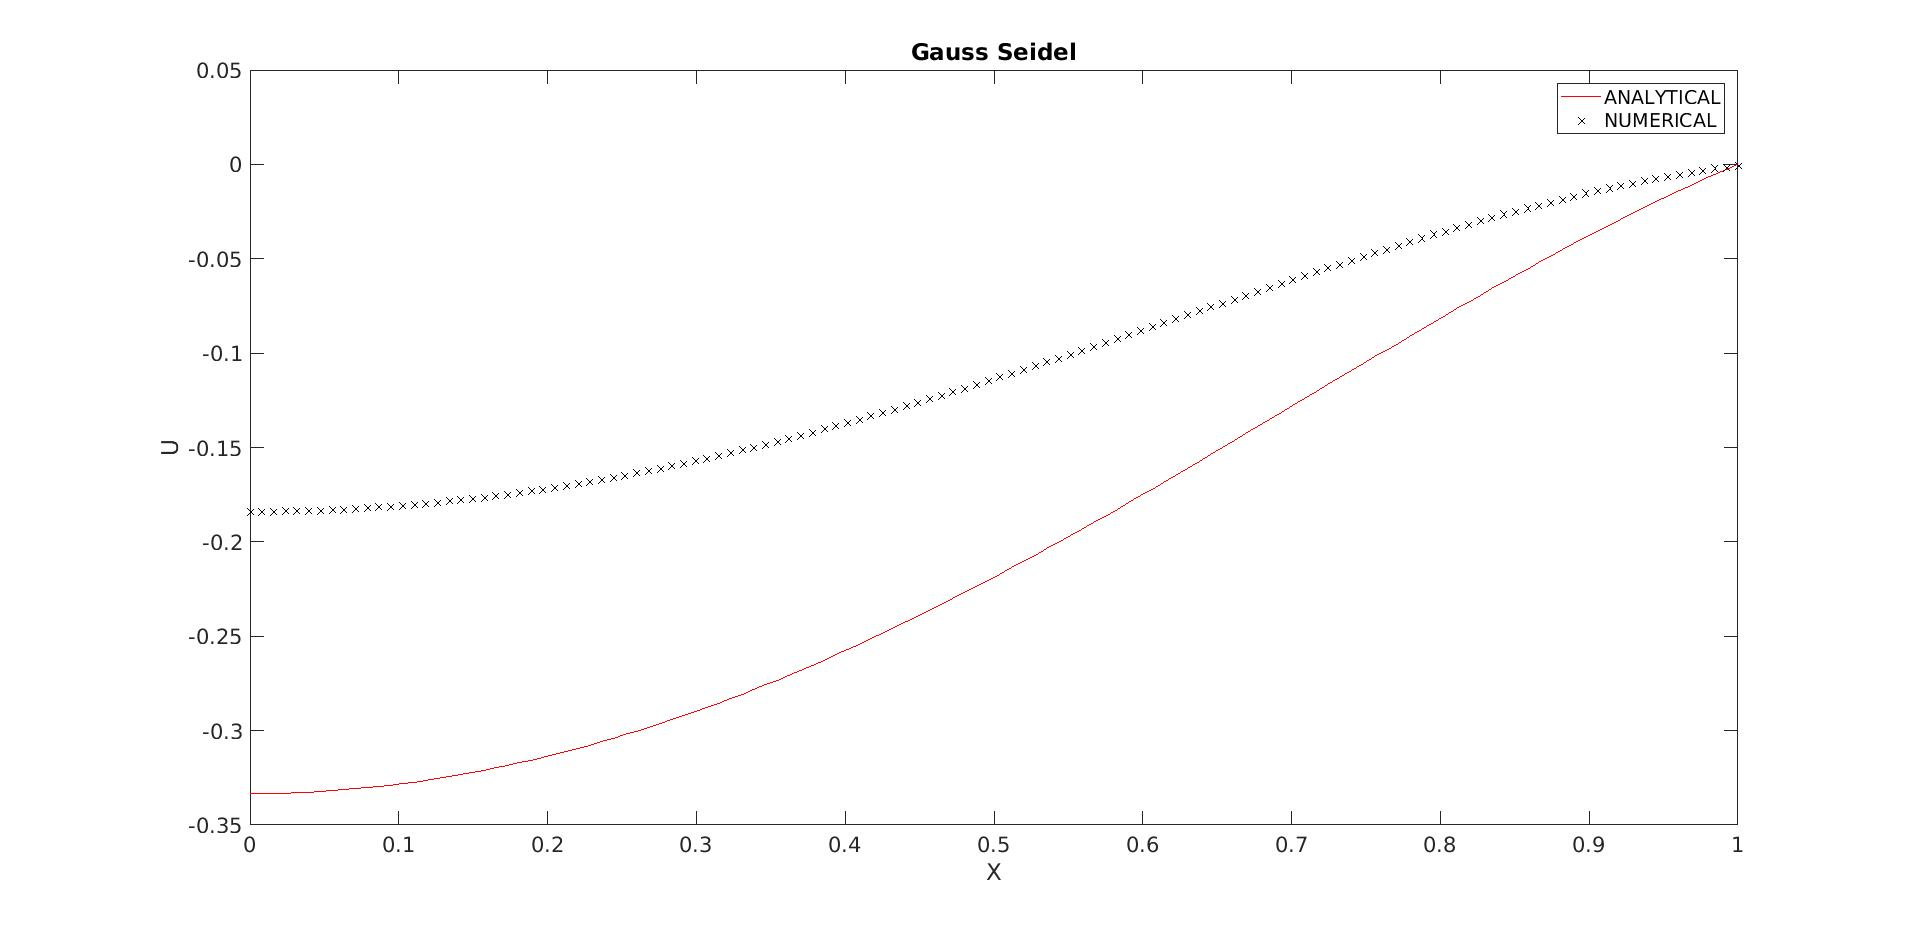
\includegraphics[width=\linewidth]{GS.jpg}
	
	
	\caption{Analytical vs Numerical Solution for Gauss Seidel method at 5000 iterations}
	\end{figure}

	\begin{figure}[H]
	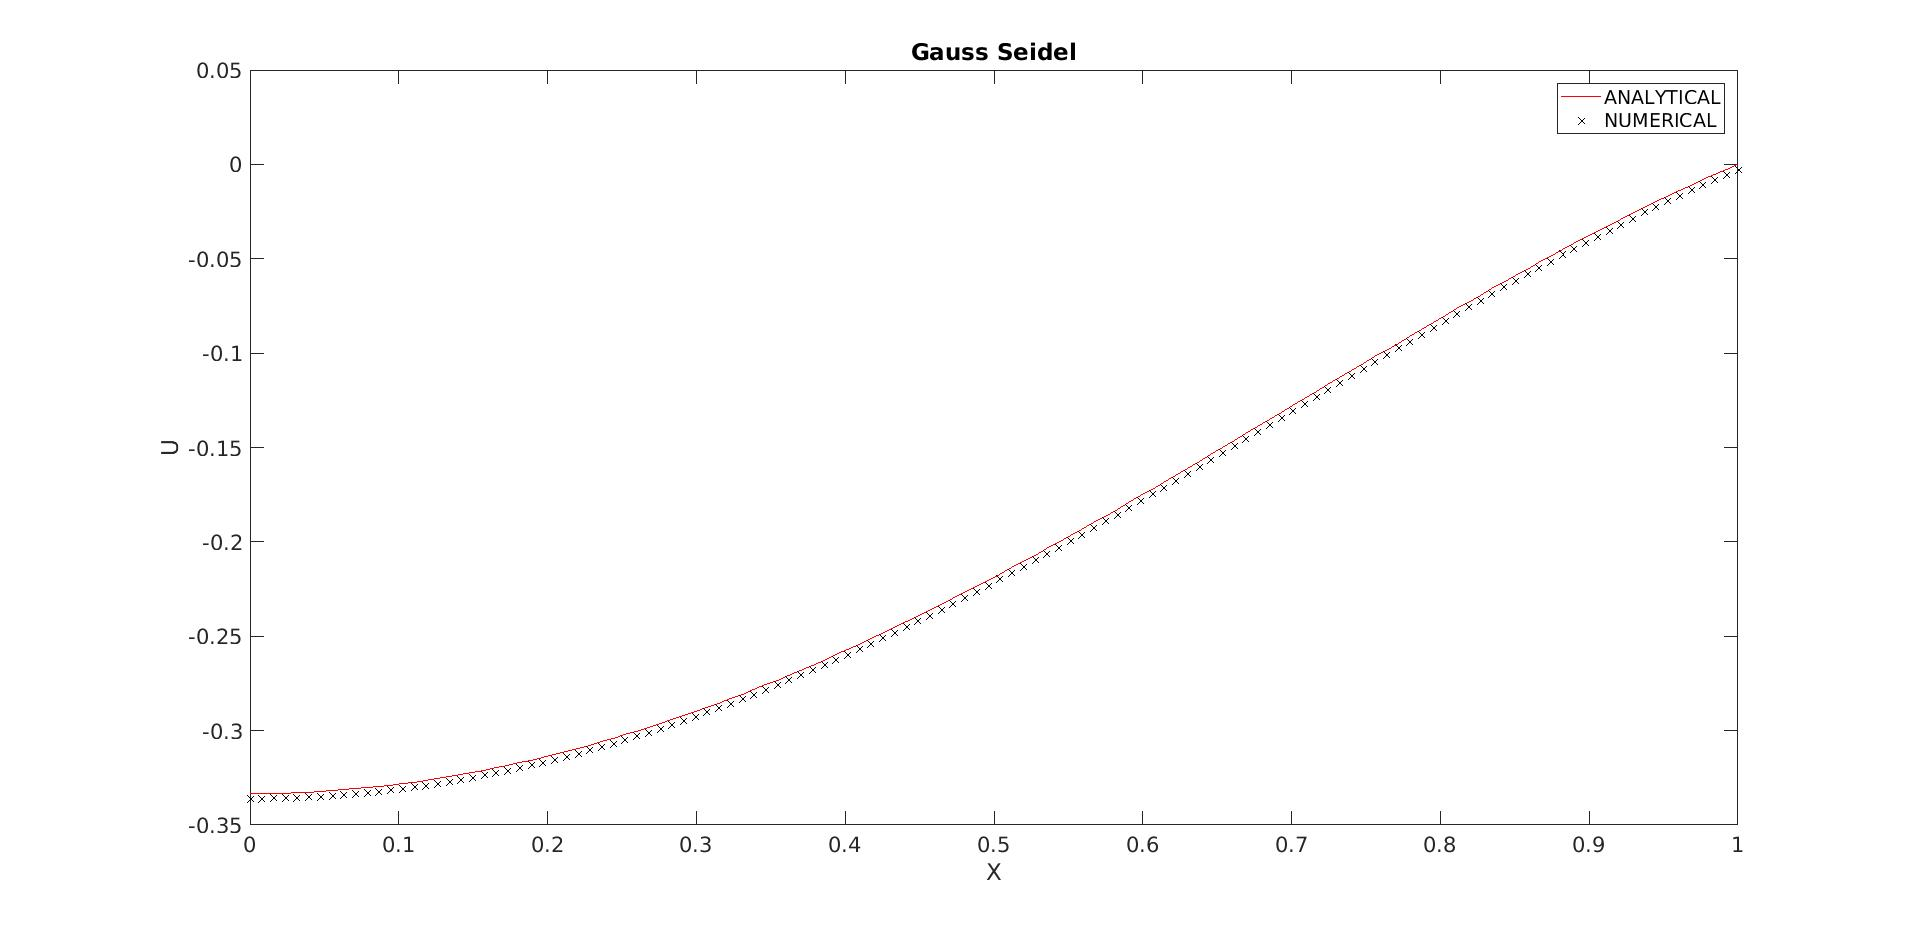
\includegraphics[width=\linewidth]{GS_50k.jpg}
	
	
	\caption{Analytical vs Numerical Solution for Gauss Seidel method at 50,000 iterations}
	\end{figure}


	The error distributions are plotted below for 5000 iterations and 50,000 iterations: 
	
	\begin{figure}[H]
		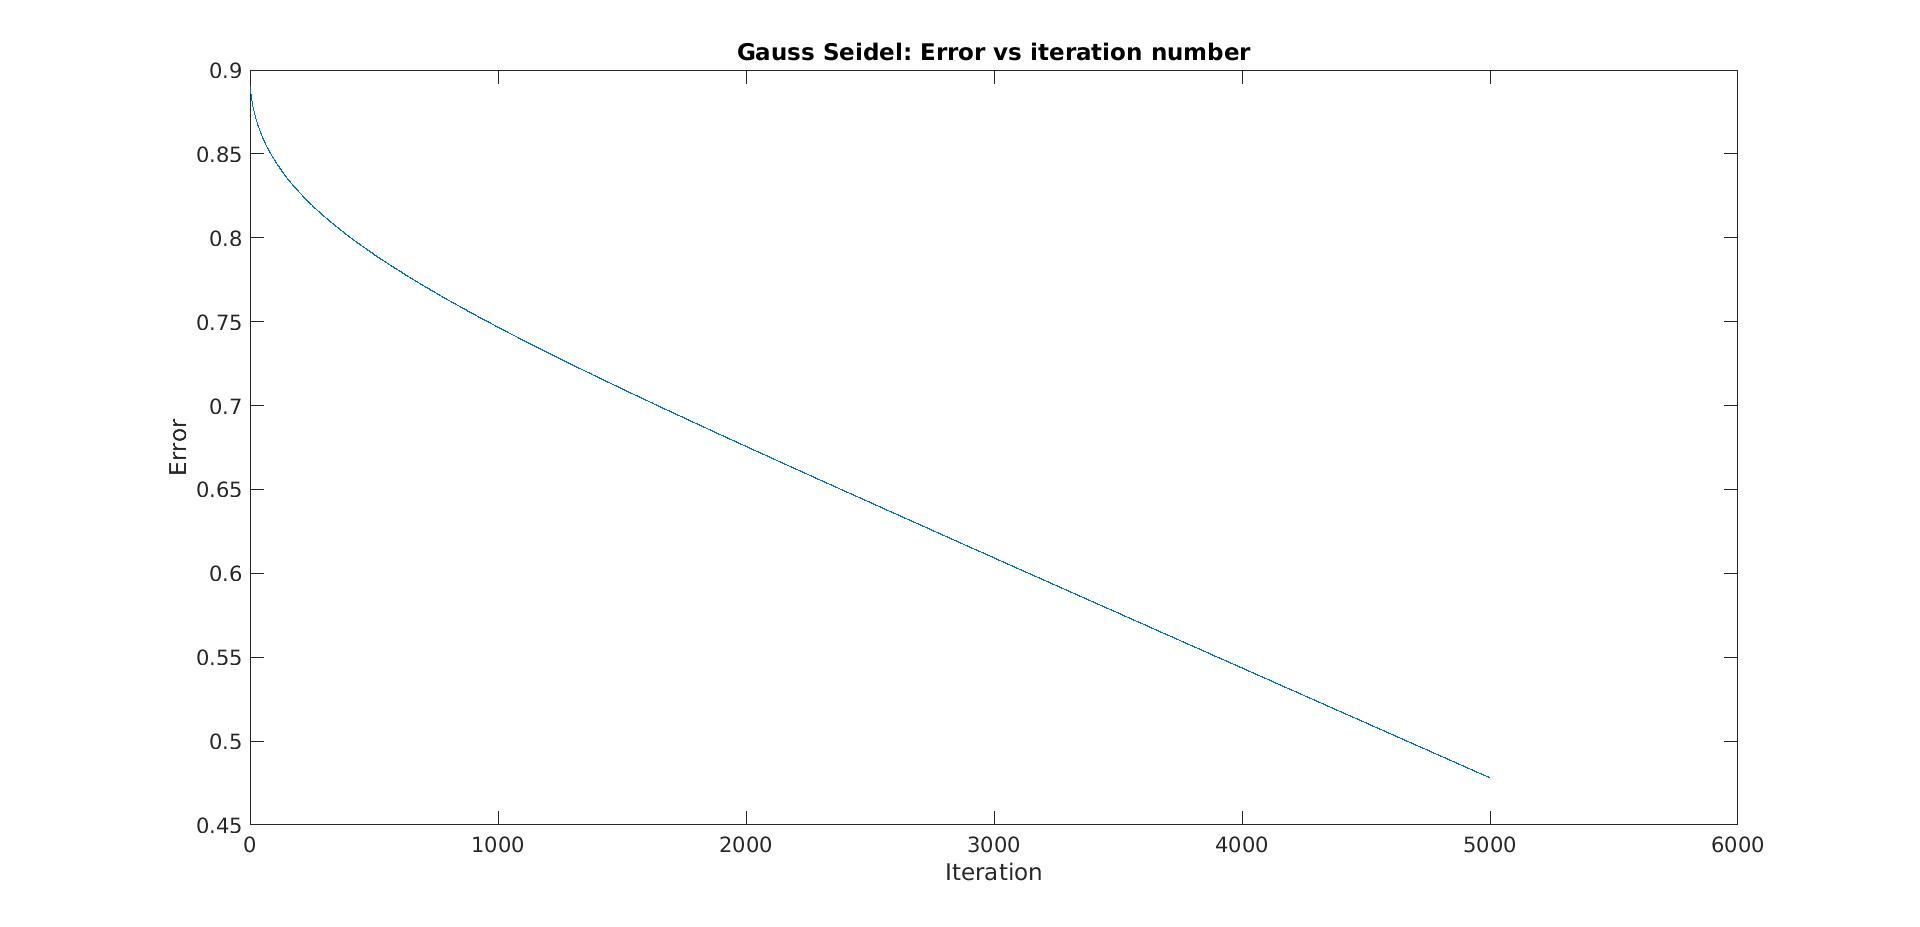
\includegraphics[width=\linewidth]{GS_error.jpg}	
		
		\caption{Error distribution for Gauss Seidel at 5000 iterations}
	\end{figure}


	\begin{figure}[H]
		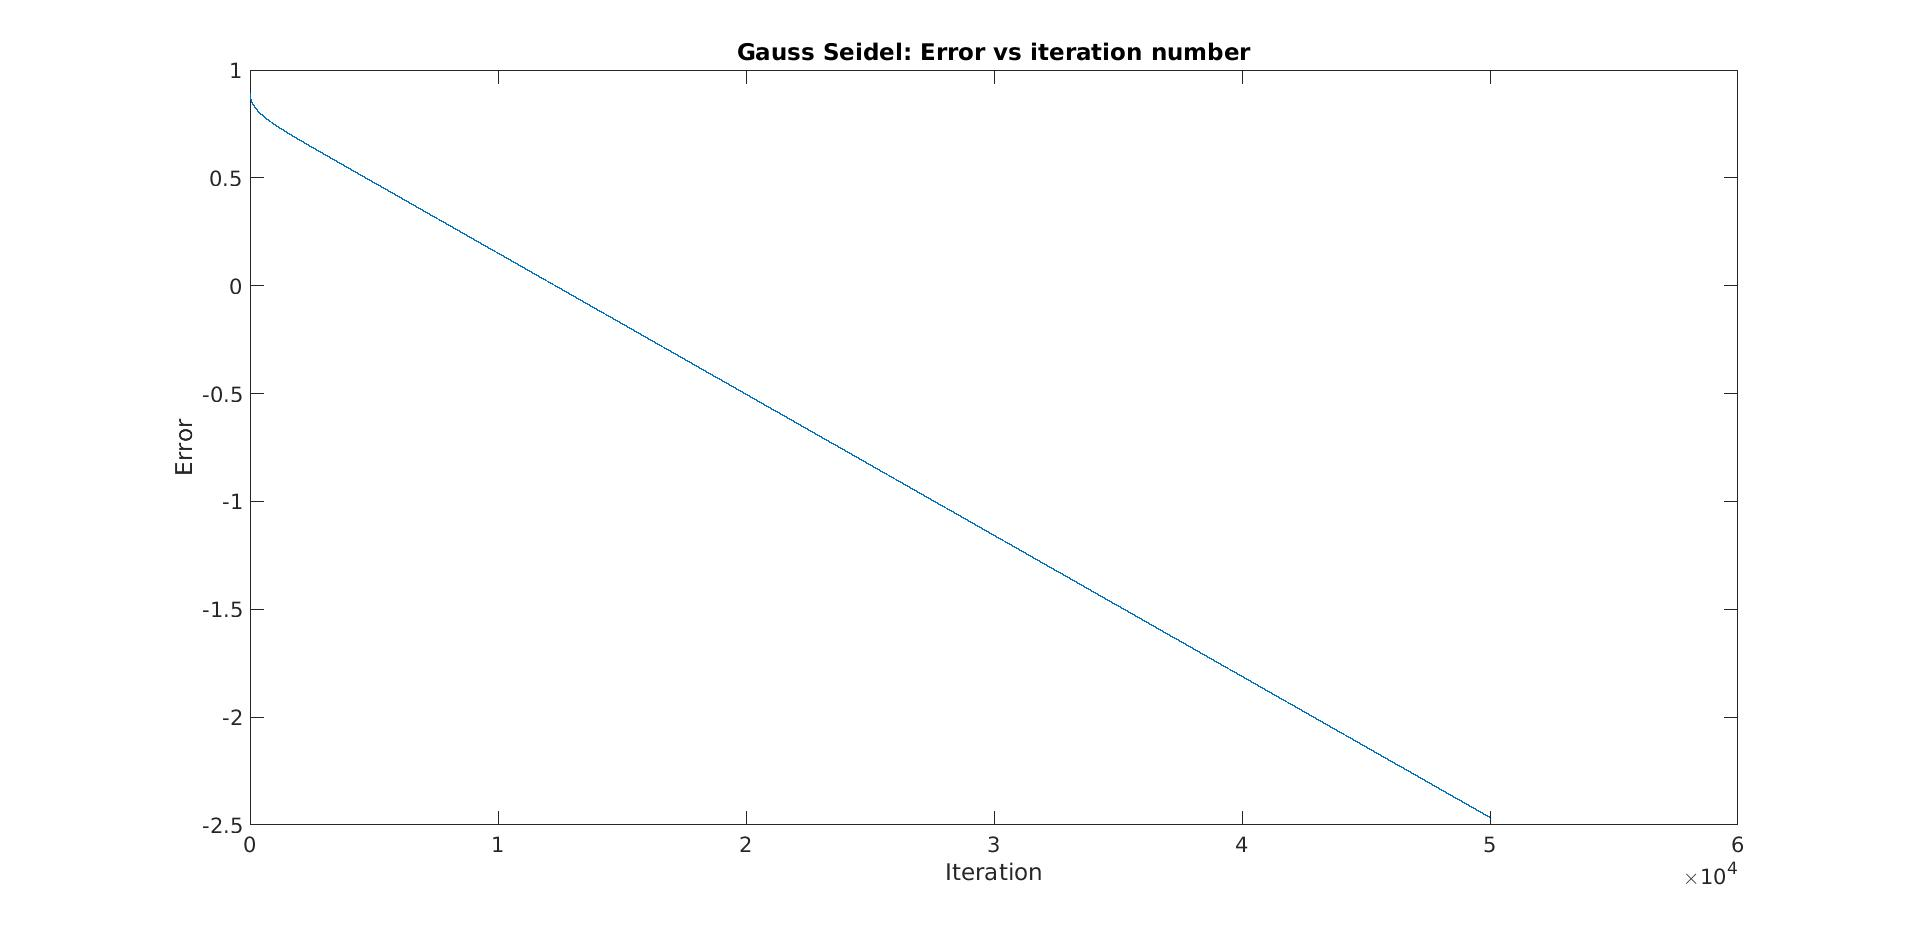
\includegraphics[width=\linewidth]{GS_error_50k.jpg}	
		
		\caption{Error distribution for Gauss Seidel at 50,000 iterations}
	\end{figure}

	\noindent
	We can see that in Figure 1, the numerical solution is getting closer to the analytical, however, it still needs more iterations to converge. In Figure 2, the result is very good because the numerical almost matches the analytical one. For the error distributions, we can see in Figure 3 that originally, the solution takes around 5000 iteration for the error to drop down.  At 50,000 iterations (Figure 4), we can see clearly, that higher iterations will help the solution to converge. This, of course, is only true if our initial guesses are not too far of from the analytical solution.
	
	  	

\subsection{Convergent Analysis}

Let $e_{k} = u - u_k$, where u is the exact solution and $u_k$ is the numerical solution. Then we can subtract the numerical solution from the exact solution  



\section{Conjugate Gradient Method without Preconditioner}



\subsection{Results}
\subsection{Convergent Analysis}
\section{Conjugate Gradient Method with Incomplete Cholesky Decomposition}
\subsection{Results}
\subsection{Convergent Analysis}
\end{document}
